
\section{Discussion} \label{sec:discussion}

\subsection{Natural vs. potential local resource}

\begin{itemize}
\item $R_{L_*} > R_{L_\circ}$, because:
  \begin{itemize}
  \item source terms are larger when starting with no-waves \note{Is this always true?}
  \item Or is it because sometimes the winds blow {\em against} the waves?
  \end{itemize}
\item Because $R_{L_*} > R_{L_\circ}$, there is an argument for defining $R_L = R_{L_*}$. However, we use it as an upper-bound (with $R_{L_\circ}$ as the lower-bound) because:
  \begin{itemize}
  \item Frequency dependence of natural vs. potential. Natural has lower-frequency peak frequency \note{(right?)}, which means it is more likely to be useful energy. I.E. most of the `extra energy' in potential is rather high-frequency so maybe not so useful?
  \item Also, $R_{L_*}$ is {\em so hypothetical} that it is rather unrealistic.
  \item Is there an argument here relating to uncertainty in source terms, or is that a {\em different} source of uncertainty?
  \end{itemize}
\item What about saying something about the cases where we extracted 
\end{itemize}

There is also a discussion here somewhere about the use of all source-terms, not just $S_{in}$. I think this also relates to the discussion above about whether $R_L = R_{L_*}$ or $R_{L_\circ} < R_L < R_{L_*}$ in the sense that we are making {\em some} assumptions/decisions about what does/does-not count in the `theoretical resource'. \note{Does a discussion of these assumptions/decisions belong here, or in the {\em methods} section?}

\begin{figure}[ht]
  \centering
  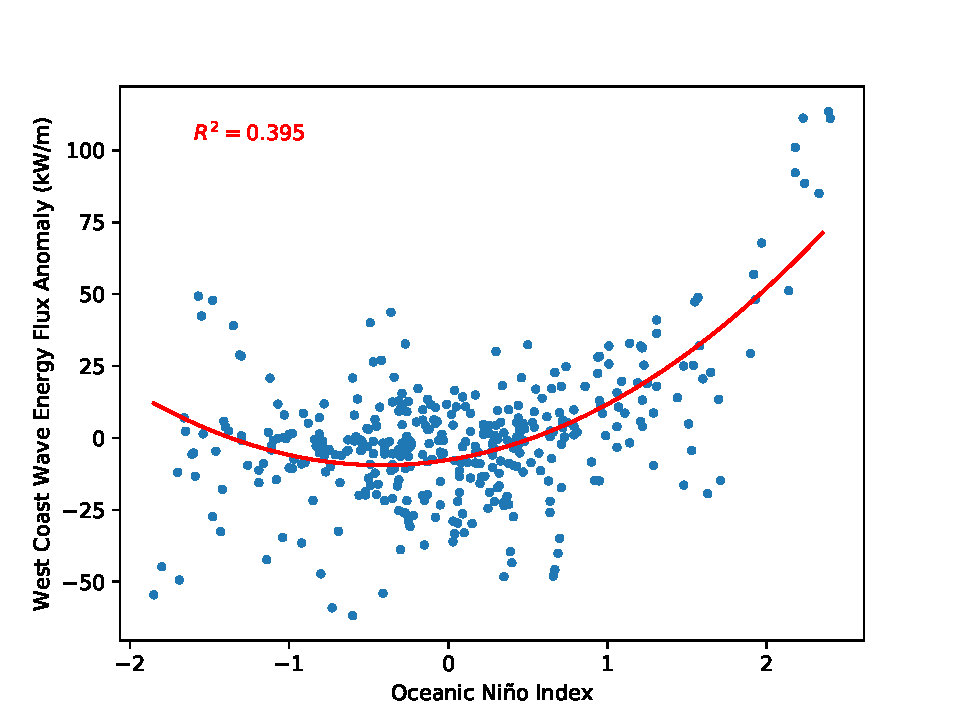
\includegraphics[width=\textwidth]{../fig/ENSO-Comparison.wc.pdf}
  \caption{West Coast wave energy flux anomaly vs. oceanic nino index. The wave energy flux anomaly (annualy cycle removed) is averaged along the EEZ boundary, has had a 5-month running average applied, and lags the ONI signal by 2-months.}
  \label{fig:wc-nino}
\end{figure}

\section{Conclusion} \label{sec:conclusion}

\begin{itemize}
\item This approach captures both local and remote resource
\item ‘Best estimate’ of total U.S. wave resource is XXX TWh/yr
\item This is theoretical, not ‘technical’ resource.
\item Combine theoretical resource estimates with device data to estimate ‘technical potential’ (AEP) for a project. i.e., this looks at methods to improve IEC standards based on this work.
\item The remote results are closer to the EPRI 2004 resource assessment results, which utilized wave directionality and the EEZ boundary.
\end{itemize}


%%% Local Variables:
%%% TeX-master: "wave_res"
%%% End:
